% !TEX root = ../Dissertation.tex
% !TEX spellcheck = en_US

\noindent 

\section {Augmented ESNet Topology}
%figure 1
ESnet is the department of Energy's dedicated science network, helping researchers meet their goals. scientific data flows are like enormous elephants. ESnet is optimized to help those elephants move quickly and efficiently around the world, so that scientists can pursue discoveries.

\begin{figure}[hbt!]
\centering
\includegraphics[width=15cm, height=10cm, page=18]{fig12.png}
\caption{Augmented ESnet Topology}
\label{fig:esnetTopo}
\end{figure}


\indent ESNet can move data at the speed of 100 gigabits per second. More than 40 percent of the links are 100 gigabits per second (precisely 34 in the above topology out of 73) and rest 10 Gbps and one of them being 40 Gbps. The following assumptions and modifications were made about the network in this research,

\begin{enumerate} [leftmargin=*]
\item Almost all the blocking happens inside the network due to the insufficient bandwidth. It is also assumed that there are enough vlan tags available for all the generated requests in the entire period of simulation.   
\item Links that could not support giant flows were taken out of the topology because most of them were used for management purposes. 
\item The Bandwidth of access ports of switches (the entry point to the network) were all set to 100 Gbps to avoid blocking at the fixtures. This makes sure that all the blocking only happens inside the domain.
\item The topology is assumed to have a bidirectional links.
\end{enumerate}

\footnote {OSCARS 1.0 is being deployed in Energy Science network}

\section {Traffic Generation}

Source traffic modeling and traffic generation is a very important aspect of research about network communication. An accurate estimation to the network traffic is the basis to handle/control the traffic. A good estimation to network traffic (PDF, CDF, mean, variance, etc..,) helps to solve the questions in the design of routing algorithm. Also, it provides a powerful and flexible tool to test all kinds of service designed for network communication. 

\indent Many works have been done in this area and the approaches cover every aspect of internet traffic. Although it is hard to dig deep into most popular questions about traffic modeling and generation. That said, this research still does its best to discuss some characteristics of internet traffic particularly in optical networks, some important distributions used to describe different aspects of traffic [1].

\subsection {Traffic Modelling}
Traffic generation and traffic modeling are two sides of a coin. A good traffic model is the goal to develop a detailed understanding of the traffic characteristics of the network. Analysis of the traffic provides information like the blocking probability for various load, the bandwidth requirements, traffic flow from a source to destination for a type of traffic (Unicast, Anycast, Manycast) and numerous other details. Also, traffic models enable network designers to make assumptions about the networks being designed based on experience and enable prediction of reservation performance for future requirements [2].

\indent A good model demands a closest approximation to the input traffic parameters such as arrival and holding time, bandwidth, source and destination for a request and their corresponding distributions. Let's inspect these parameters one at a time.

\subsubsection {Arrival time distribution}
The Poisson process is an extremely useful process for modeling purposes in many practical applications, such as, for example, to model arrival processes for queueing models. It is empirically found that in many circumstances the arising stochastic processes can be well approximated by a Poisson process. 
Hence under these conditions, the arrival processes can be modeled as Poisson,
\begin{enumerate} [leftmargin=*]
\item Each request has to be independent to each other.
\item At any time, only one request can arrive (ie. Only one can be served at a time while the other is waiting in the queue).
\item For any given time frame, the probability of arrivals of certain time interval is the same for all time intervals of equal length 
\end{enumerate}

\indent From the standpoint of the network users, the requests are typically triggered by a particular events. But from the standpoint of the network, these request initiations are somewhat arbitrary and unpredictable. Therefore, the sequence of times at which requests arrive is a random process. Moreover, these requests are triggered by different users that has no relation to each other. To make this assumption further stronger, each request has to be treated one by one based on first come first serve and this seems to acknowledge the orderliness property. Also, the requests arriving to OSCARS will be processed one by one. Since our problem in hand uphold the properties of Poisson, it has been considered in our work [2].

\begin{enumerate}[label=(\alph*),leftmargin=*]
\item\textit {Poisson Arrival Process}
	
Now that we have established scenarios where we can assume an arrival process to be Poisson. Let's look at the probability density function of exponential arrival . 

\begin{figure}[H]
\centering
\includegraphics[width=12cm, height=08cm, page=20]{fig13.png}
\caption{Exponential PDF}
\label{fig:expoPDF}
\end{figure}	
	
\hspace{5mm}  An interesting observation in Poisson models is that as the mean increases (lambda is more than 30), the properties of the Poisson distribution approach those of the normal distribution.

\hspace{5mm} It is also observed that the time between any two arrivals follow exponential distribution. When events occur according to an exponential distribution, they are said to occur completely at random. Thus, the arrival time of the next event is not affected by the time elapsed since the previous event. 

\item\textit{Single Controller criteria}

With M/M/1 queueing system, we have a single server for the queue [3]. Hence, M/M/1 can be applied to our system since it meets our criteria of single controller for requests from one network domain.
\end{enumerate}

\subsubsection {Exponential Service Times}
In an M/M/1 queueing system we assume that service times for customers are also exponentially distributed (i.e. generated by a Poisson process). Unfortunately, this assumption is not as general as the arrival time distribution. But it could still be a reasonable assumption when no other data is available about service times which in our case its true.


\begin{enumerate}[label=(\alph*),leftmargin=*]
\item Calculation of Load \\
Load or Traffic Intensity, is defined as the average arrival rate (lambda) divided by the average service rate (mu).

Load = Lambda / mu; (Load $>=$ 0)

while	 Lambda- Average Arrival rate
mu- Average Service rate
\end{enumerate}	

\footnote {Choice of load value is very critical for the analysis of traffic. From the above equation if arrival increases, the load on the network also increases (there should be more active requests in the network).} 

\subsubsection{ Bandwidth Distribution}
From [5], it is true that the commercial network has diversified request bandwidths. The more appropriate distribution in this case follows uniform distribution considering the range of usage of network in question. However, this generalized assumption cannot be valid for ESnet. As explained in the previous sections, ESnet is a high-speed network engineered and optimized to support large-scale transfer [8]. It is also understood that it is carrying data that is twice the rate of the commercial Internet; today it carries approximately 20 petabytes of data each month.  Hence, uniform distribution of bandwidth may lead to inaccurate results as most of the links are 100 Gbps and the range of usage is not clearly known. 

\indent Any alternatives here? It is also inferred from [4] that ESnet differs from a traditional provider of network services because massive science data flows require different handling than small flows generated on the global Internet. This makes it certain that most of the requests for ESnet may demand high bandwidth as they arrive. This offers an ascend to consider normal distribution for the choice of bandwidth for each request. Meanwhile, this does not provide any assurance for realistic traffics except that it is more appropriate than uniform distribution in our case. That said, the realistic bandwidth distribution may not fit to any general distribution because it requires more intensive research based on the traffic monitoring.

The following is the plot of the standard normal probability density function \\
\begin{figure}[H]
\centering
\includegraphics[width=10cm, height=08cm, page=23]{fig14.png}
\caption{PDF of Normal Distribution}
\label{fig:normalPDF}
\end{figure}
 
\subsubsection {Device Distribution}
Unlike bandwidth, vendor, unfortunately did not provide further statistics on how these traffic flows are distributed in the network because they form business critical information. Due to this reason, it is safe to consider uniform distribution as load may be equally distributed across all fixtures when number of requests approach higher values.
The probability density function of the uniform distribution is given by,
 
$f(x)=1/b-a$ ; for $0< x< 1$

\begin{figure}[H]
\centering
\includegraphics[width=10cm, height=08cm, page=24]{fig15.png}
\caption{PDF of Uniform Distribution}
\label{fig:unifirmPDF}
\end{figure}

\subsection {Input parameters for traffic generation}
To determine a realistic performance evaluation, the input load is carefully chosen to keep the blocking probability closer to the working range as much as possible. It is highly unlikely that a network of such capacity be used for high blocking for dynamic traffic generation. Moreover, the topology is frequently being updated by ESNet to support the high volume of network as the demand increases. Because of these reasons, strenuous testing for very high loads of traffic is avoided. 

\indent Repeated trials and accurate examinations have been made to fix a proper load range to achieve the above. Also, the traffic generation parameters are carefully chosen to match the realistic traffic generated to controller OSCARS handling ESNet. For example, OSCARS is responsible for approximately 5,000 virtual circuit reservations created for demos, transient experiments, and projects [7]. This detail on number of requests over the simulation period is considered for this research and it puts optimum efforts to adjust the load accordingly. It is also crucial that simulator needs to run for more number of small, realistic traffic sets to realize the optimal results. Also, the request bandwidths vary based on the type of traffic flows and follows normal distribution as discussed in the section 3.2.1.3. 
%table 1
\begin{table}[!htbp]
\centering
\caption{Traffic Distribution Summary}
 	\begin{tabular}{|c|c|c|}
	\hline\hline
	\textbf{Traffic Parameter} & \textbf{Value} & \textbf{Distribution}\\
	\hline
	Bandwidth&1 Gbps  (variant of 400 Mbps)&Normal\\
	Device&(S,D) =$> (0, 34)&Uniform\\
	Ports in the device&Varies based on devices&Uniform\\
	Start Time&(-ln U/lambda) &Discrete Poisson\\
	End Time&Start time + (-ln U/mu) &Exponential\\
	\hline
	\end{tabular}
\end{table}


 \indent All results shown in this chapter represent the average of 10 unique sets of reservation requests, and we have included the 95\% confidence intervals, which are quite narrow.

